
%(BEGIN_QUESTION)
% Copyright 2006, Tony R. Kuphaldt, released under the Creative Commons Attribution License (v 1.0)
% This means you may do almost anything with this work of mine, so long as you give me proper credit

Suppose we were to equip an electric oven with the following proportional control system.  An {\it instrumentation amplifier} forms the heart of this control system, outputting a voltage proportional to the difference in voltage between the noninverting and inverting inputs.  An external resistor sets the differential gain of the amplifier:

$$\includegraphics[width=15.5cm]{i01456x03.eps}$$

Measuring temperature over time with a {\it recorder}, suppose we see this graph of oven temperature over time:

$$\includegraphics[width=15.5cm]{i01456x01.eps}$$

The temperature slowly rises from ambient to setpoint, approaching the setpoint asymptotically (slower as it gets closer), until it finally reaches its goal.

Having the process variable accurately reach setpoint is, of course, one of the goals of a control system.  However, it is not the only goal.  Ideally, we would like to have the process variable attain setpoint {\it as quickly as possible}.  How could the proportioning control be modified to increase the response time of the control system from what is shown here?  What would have to be changed or altered so that the proportional control took faster action to reach setpoint?

Hint: analyze the problem from the perspective of the system's current behavior.  What would a proportional control system be doing wrong that would make the process variable approach setpoint so slowly?  Imagine riding in an automobile with a driver who was very slow to correct lane position or speed.  What would a good driver do that is different from the behavior of a slow-acting driver?
 
\underbar{file i01456}
%(END_QUESTION)





%(BEGIN_ANSWER)

The problem with this control system is that its output does not respond aggressively enough to changes in the input.  What we need is a controller that saturates (100\% output signal to the heater control transistor) while the temperature is substantially below setpoint, and begins to ``throttle'' only when we come near setpoint.  

I will let you determine what needs to be changed in this circuit to improve its control behavior!  

%(END_ANSWER)





%(BEGIN_NOTES)

To improve the response time of this proportional control system, we must increase the voltage gain of the differential amplifier.  If we make this change to the control circuit, we will see an improvement in control response that looks something like this:

$$\includegraphics[width=15.5cm]{i01456x02.eps}$$

\vskip 20pt \vbox{\hrule \hbox{\strut \vrule{} {\bf Virtual Troubleshooting} \vrule} \hrule}

This question is a good candidate for a ``Virtual Troubleshooting'' exercise.  Presenting the diagram to students, you first imagine in your own mind a particular fault in the system.  Then, you present one or more symptoms of that fault (something noticeable by an operator or other user of the system).  Students then propose various diagnostic tests to perform on this system to identify the nature and location of the fault, as though they were technicians trying to troubleshoot the problem.  Your job is to tell them what the result(s) would be for each of the proposed diagnostic tests, documenting those results where all the students can see.

During and after the exercise, it is good to ask students follow-up questions such as:

\begin{itemize}
\item{} What does the result of the last diagnostic test tell you about the fault?
\item{} Suppose the results of the last diagnostic test were different.  What then would that result tell you about the fault?
\item{} Is the last diagnostic test the best one we could do?
\item{} What would be the ideal order of tests, to diagnose the problem in as few steps as possible?
\end{itemize}


%INDEX% Control, proportional: controller gain

%(END_NOTES)


